82. $\cfrac{(x^2+3x-18)\sqrt{5-x}}{1-x}\geqslant0\Leftrightarrow\cfrac{(x+6)(x-3)\sqrt{5-x}}{1-x}\geqslant0.$ Применив метод интервалов, найдём ответ: $x\in(-\infty;-6]\cup(1;3)\cup\{5\}.$
\begin{figure}[ht!]
\center{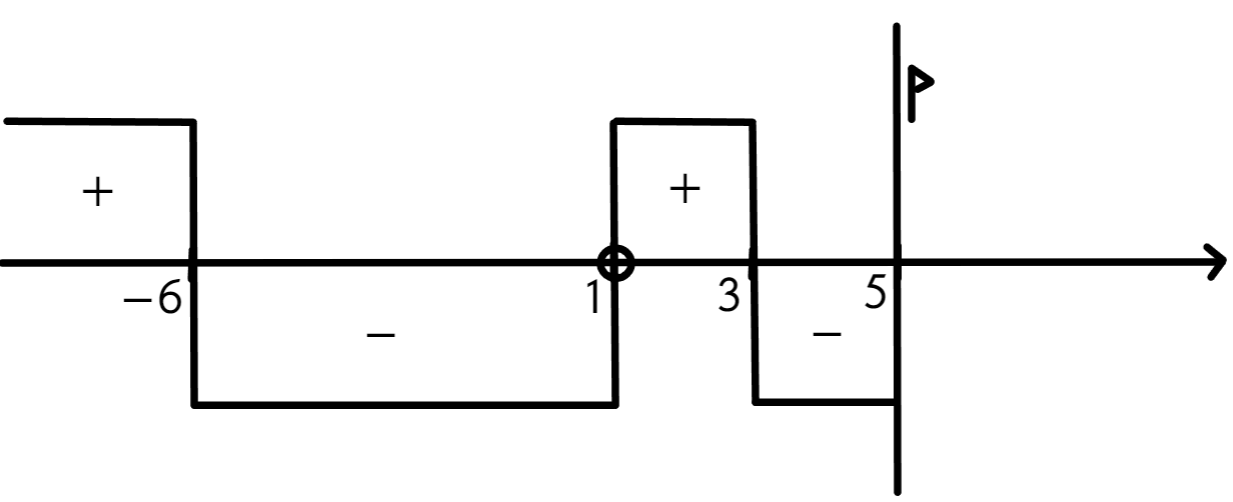
\includegraphics[scale=0.35]{ner9-83.png}}
\end{figure}\\
